\documentclass{article}
\usepackage[utf8]{inputenc}
\usepackage{graphicx}
\usepackage{algpseudocode}
\usepackage{caption}
\usepackage{algorithm}



\title{Iskanje najdaljse poti na kaktusih}
\author{Vid Treven}
\date{December 2022}

\begin{document}

\maketitle

\section{Potrebne definicije}

\textbf{Kaktus} (tudi kaktusovo drevo) je povezan graf, za katerega velja da imata katerakoli dva cikla tega grafa najvec eno skupno vozlisce. Ekvivalentna definicija se glasi: Kaktus je povezan graf, katerega vsaka povezava je v najvec enemu ciklu. \textbf{Korenski kaktus} je kaktus, ki ima eno izmed vozlisc za koreno. \\
\textbf{Ciklicna vrsta} je vrsta A[1,...,n], za katero velja: 
\begin{enumerate}
    \item $n \geq 3$
    \item $A[1]$ in $A[n]$ sta soseda v tej vrsti
\end{enumerate}
V kontekstu ciklicnih vrst je \textbf{razdalja} definirana kot \\ D$(i,j)$ = max $\{|i-j|, n-|i-j|\}$ \\
Naj bo $G$ korenski kaktus s korenom $u$. Recimo, da je koreno u vozlisce v $r$ ciklih $s_1, s_2, ..., s_r$. Ce izbrisemo koreno $u$ dobimo $d+r$ povezanih komponent. Te komponente so \textbf{minion-i}. $d$ minion-om, ki so z vozliscem $u$ povezani z enojnimi povezavami pravimo \textbf{drevesni minion-i}, ostalim $r$ pa \textbf{ciklicni minion-i}. Vsak drevesni minion je spet korenski kaktus, cigar koreno je vozlisce, povezano z $u$-jem. To pa ne velja za ciklicne minione. V vsakem ciklicnem minionu $H_i$ je pot $s_i - u$ \textbf{baza} (V nasem primeru je baza za $H_1$ je $w_1^1, w_2^1, ..., w^1_{t_1}$). Korena drevesnih minionov so \textbf{drevesni otroci u-ja}. Drevesni otroci ter vozlisca v bazah ciklicnih minionov so \textbf{otroci u-ja} (V nasem primeru so drevesni otroci $u$-ja $v_1, ... ,v_d$, otroci $u$-ja pa so $v_1, ..., v_d, w_1^1, ..., w^1_{t_1}, ..., w_1^2, ..., w^2_{t_2}$). Vozliscu brez otrok pravimo \textbf{list}.

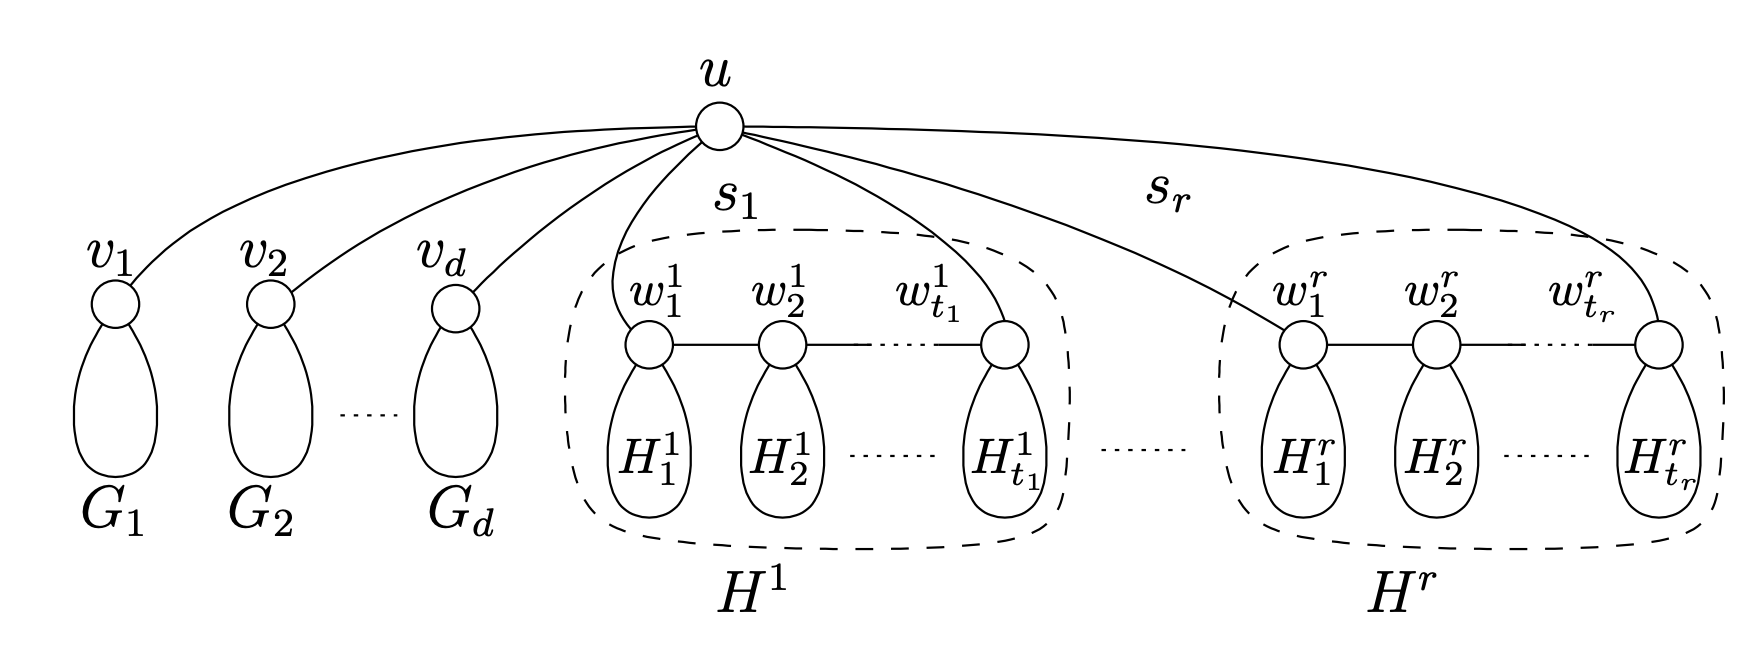
\includegraphics[width=330pt]{kaktus.png}

\section{Algoritem}

Algoritem za iskanje najdaljse poti v kaktusih deluje po principu deli in vladaj, torej velik problem se razdeli na vec manjsih problemov, ki so lazje resljivi. Osnovni algoritem NAJDALJSI KAKTUS izbere koren u in poklice funkcijo NAJDALJSI KORENSKI KAKTUS. Ta algoritem vrne dve stevili. Prvo ($l_1(u)$) predstavlja dolzino najdaljse poti v podkaktusu s korenom $u$, drugo ($l_2(u)$) pa je enako najdaljsi poti v podkaktusu s korenom $u$, katere koncno vozlisce je $u$. Algoritem deluje tako, da zacetni graf razdeli na manjse podgrafe (minione) in na njih spet izvede algoritem NAJDALJSI KORENSKI KAKTUS. Za ciklicne minione uporabimo se algoritem AUX, ki v ciklicni vrsti poisce najdaljso pot (razdaljo med dvema vozliscema $+$ njuno $l_2$).

\begin{algorithm}
\begin{algorithmic}[1]
\caption{NAJDALJSI KAKTUS(G)}
\State Izberi katerokoli vozlisce $u$ na grafu $G$
\State Predstavi graf $G$ kot korenski kaktus s korenom $u$
\State NAJDALJSI KORENSKI KAKTUS(G[u], u)
\State \Return $l_1(u)$
\end{algorithmic}
\end{algorithm}

\begin{algorithm}
\begin{algorithmic}[1]
\caption{NAJDALJSI KORENSKI KAKTUS(G[u], u)}
\If{$u$ je list}
    \State $(l_1(u), l_2(u)) = (0,0)$
\Else
    \State drevesni otroci $u$-ja so $v_1, ..., v_d$
    \State ciklicni minioni $u$-ja so $H^1, ..., H^r$
    \State baza za $H^i$ je $w_1^i, w_2^i, ..., w^i_{t_1}$
    \For{$u$-jev otrok $a$} 
        \State NAJDALJSI KORENSKI KAKTUS(G[a], a)
    \EndFor
    \State $P = \{l_2(v_i) + 1|1 \leq i \leq d\}_M$
    \For{$1 \leq i \leq r$}
        \State $q_i = max\{l_2(w^i_k) + max\{k, t_i-k+1\}|1\leq k \leq t_i$
    \EndFor
    \State $Q = \{q_i|1 \leq i \leq r\}_M$
    \For{$1 \leq i \leq r$}
        \State $z_i$ = AUX$(A[0, l_2(w_1^i), ..., l_2(w^i_{t_1})])$
    \EndFor
    \State $x$ = max$\{ P \cup Q \}_M$
    \State $y$ = second-max$\{ P \cup Q \}_M$
    \State $z$ = max$\{z_i|1 \leq i \leq r\}_M$
    \State $m$ = max$\{l_1(a)| a$ je otrok $u$-ja$\}_M$
    \State $l_1(u)$ = max$\{x+y, z, m \}$
    \State $l_2(u)$ = $x$
\EndIf
\end{algorithmic}
\end{algorithm}

\begin{algorithm}
\begin{algorithmic}[1]
\caption{AUX(A[1...n])}
\State $B[0...n]$ in $C[1...n]$ naj bosta linearni vrsti
\State $B[0] = 0$
\For{$1 \leq i \leq n$} 
        \State $B[i] = max\{ B[i-1], A[i] - (i-1) \}$
        \State $C[i] = B[i-1] + A[i] + (i-1)$
\EndFor
\State $x$ = max$\{ C[i]|1 \leq i \leq n \}$
\For{$1 \leq i \leq n$} 
        \State $B[i] = max\{ B[i-1], A[i] + (i-1) \}$
\EndFor
\State $C[n] = A[n] + 1$
\For{$1 \leq i \leq n$} 
        \State $C[i] = max\{ C[i+1], A[i] + n - (i-1) \}$
\EndFor
\State $y$ = max$\{ B[i] + C[i+1]| 1 \leq i \leq n-1 \}$
\State \Return max$\{ x,y \}$
\end{algorithmic}
\end{algorithm}


\end{document}
